\chapter{Proposed Solution}

\section{Problem Formulation}

Let $\mathcal{I} = \{I_i\}_{i=1}^N$ be a set of calibrated multi-view images with known camera poses obtained from Structure-from-Motion.
The goal is to reconstruct a geometrically consistent scene representation using a set of Gaussian primitives:

\begin{equation}
\mathcal{G} = \{ g_k \}_{k=1}^K,
\end{equation}

where each Gaussian $g_k$ is parameterized by its center $\mathbf{x}_k \in \mathbb{R}^3$, covariance $\Sigma_k$, opacity $\alpha_k$, and color features.

The standard 3D Gaussian Splatting formulation optimizes parameters by minimizing photometric reconstruction error:

\begin{equation}
\mathcal{L}_{photo} =
\sum_{i=1}^{N}
\left\|
R(\mathcal{G}, \Pi_i) - I_i
\right\|_2^2,
\end{equation}

where $R(\cdot)$ denotes the differentiable renderer and $\Pi_i$ is the projection associated with camera $i$.

However, purely photometric supervision is insufficient in:

\begin{itemize}
    \item textureless planar regions,
    \item areas with weak gradients,
    \item geometrically ambiguous boundaries.
\end{itemize}

This often leads to over-densification, floating artifacts, and inconsistent surface normals.

To address these limitations, we introduce geometry-aware regularization and adaptive primitive allocation into the optimization process.

The final objective becomes:

\begin{equation}
\mathcal{L} =
\mathcal{L}_{photo}
+
\lambda_d \mathcal{L}_{depth}
+
\lambda_n \mathcal{L}_{normal}
+
\lambda_p \mathcal{L}_{planar}
+
\lambda_e \mathcal{L}_{edge},
\end{equation}

\noindent where $\lambda_d$ weights the depth prior described in Section~\ref{sec:depth_prior}, $\lambda_n$ weights the normal prior described in Section~\ref{sec:normal_prior}, $\lambda_p$ weights the planar regularization described in Section~\ref{sec:planar_prior}, and $\lambda_e$ weights the edge-aware normal reinforcement described in Section~\ref{sec:edge_prior}.

\section{Geometric Prior Formulations}
\label{sec:geometry_priors}

While 3D Gaussian Splatting provides an explicit and efficient scene representation, its optimization is primarily driven by photometric supervision. Purely image-based supervision can lead to geometric artifacts such as floaters, inconsistent surface orientation, and poor reconstruction in textureless regions. To address these limitations, additional geometric priors are incorporated into the training process. This section introduces the general form of each prior type; their specific implementation within our framework is described in Section~\ref{sec:solution_architecture}.

\subsection{Depth Priors}

Depth priors provide direct supervision on scene geometry. Depth information can be obtained from multi-view stereo (MVS) methods, LiDAR sensors, or monocular depth estimation networks. Let $D_{render}(\mathbf{u})$ denote the depth rendered from the Gaussian representation and $D_{prior}(\mathbf{u})$ the externally estimated depth map. A common supervision term is:

\begin{equation}
\mathcal{L}_{depth}
=
\sum_{\mathbf{u} \in \Omega}
\left|
D_{render}(\mathbf{u}) - D_{prior}(\mathbf{u})
\right|,
\end{equation}

where $\Omega$ is the set of pixels with reliable depth values. Depth supervision reduces floating artifacts and stabilizes optimization in low-texture regions.

\subsection{Normal Priors}

Surface normal priors enforce orientation consistency of reconstructed surfaces. Normals can be derived from depth maps or predicted by monocular estimation networks. Let $\mathbf{n}_{render}(\mathbf{u})$ denote the rendered surface normal and $\mathbf{n}_{prior}(\mathbf{u})$ the reference normal. A cosine-similarity loss is commonly used:

\begin{equation}
\mathcal{L}_{normal}
=
\sum_{\mathbf{u}}
\left(
1 -
\mathbf{n}_{render}(\mathbf{u})^\top
\mathbf{n}_{prior}(\mathbf{u})
\right).
\end{equation}

Normal constraints improve local surface smoothness and reduce geometric noise, particularly in planar or weakly textured regions.

\subsection{Mesh-Based Priors}

When an approximate surface mesh $\mathcal{M}$ is available (e.g., reconstructed via TSDF fusion), it can serve as a geometric regularizer. Let $\text{dist}(\boldsymbol{\mu}_i, \mathcal{M})$ denote the shortest distance from the $i$-th Gaussian center to the mesh surface. The regularization term is:

\begin{equation}
\mathcal{L}_{mesh}
=
\sum_{i}
\text{dist}(\boldsymbol{\mu}_i, \mathcal{M})^2.
\end{equation}

This prior enforces surface adherence and improves global geometric consistency, and is particularly useful in structured environments where reliable coarse geometry can be extracted.

\subsection{Edge and Planar Priors}

Image edges and planar segment boundaries encode strong structural cues. Planar priors encourage Gaussians within a detected plane to share a common depth surface. Edge-aware priors spatially modulate primitive allocation: densification is boosted near structural boundaries and suppressed in homogeneous interiors. Together, these priors improve reconstruction of sharp transitions and prevent over-densification on large flat surfaces.

\section{Solution Architecture}
\label{sec:solution_architecture}

Figure~\ref{fig:unified_pipeline} presents the overall architecture of the proposed framework. The pipeline takes a set of calibrated multi-view images as input and extracts four monocular geometric priors — edges derived from plane boundaries, plane segmentation masks, dense depth maps, and surface normal maps — each of which feeds into a corresponding rendering-space loss term. These four loss terms, together with the standard photometric loss $\mathcal{L}_{rgb}$ and an optional mesh-based term $\mathcal{L}_{mesh}$, are jointly minimized during Gaussian optimization. The diagram uses color coding to distinguish component types: blue boxes represent input geometric priors, green boxes denote loss regularization terms, purple boxes indicate processing steps, and orange represents the central optimization objective.

\begin{figure}[t]
    \centering
    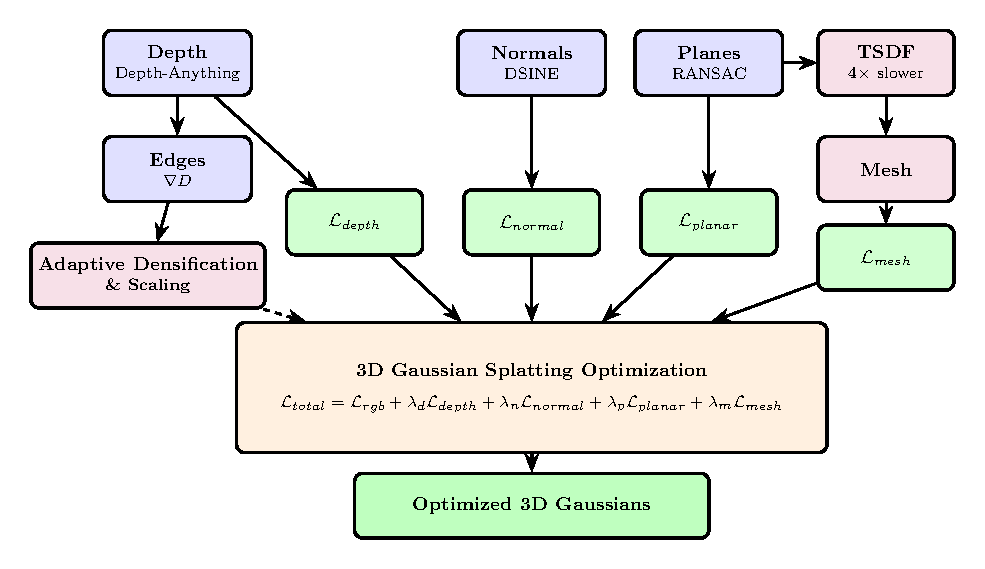
\includegraphics[width=\linewidth]{pipeline_unified.pdf}
    \caption{Unified geometry-aware 3D Gaussian Splatting framework.}
    \label{fig:unified_pipeline}
\end{figure}

The architecture extends the standard Gaussian Splatting pipeline with two complementary components:

\begin{enumerate}
    \item Geometry-aware priors operating in rendering space.
    \item Edge-aware adaptive densification for compact representation.
\end{enumerate}

\subsection{Geometry-Aware Regularization}

All geometric constraints are applied in rendering space rather than directly constraining primitive parameters. This preserves the flexibility of Gaussian primitives while enforcing global geometric consistency.

\subsubsection{Depth Prior}
\label{sec:depth_prior}

Depth prior maps $D_p$ are estimated per-view using DUST3R (Dense Unsupervised Surface Transformation via Regression), a fast monocular depth estimator. These priors are aligned with rendered depth $D_r$ to stabilize optimization in textureless regions:

\begin{equation}
\mathcal{L}_{depth}
=
\left\|
D_r - D_p
\right\|_1,
\end{equation}

reducing floating artifacts and improving geometric consistency across views.

\subsubsection{Normal Prior}
\label{sec:normal_prior}

Surface normal prior maps $N_p$ are also estimated using DUST3R per-view. These normals are regularized alongside rendered normals $N_r$:

\begin{equation}
\mathcal{L}_{normal}
=
\left\|
N_r - N_p
\right\|_1
+
\left(1 - N_r \cdot N_p \right),
\end{equation}

promoting locally coherent surface orientation and reducing normal inconsistencies.

\subsubsection{Planar Regularization}
\label{sec:planar_prior}

Planar segmentation priors are extracted from single images using SAM3 (Segment Anything Model v3), which identifies and delineates planar regions. For each segmented planar region, a plane is fitted to the rendered depth map. Let $D_{plane}$ denote the depth values induced by this fitted plane. The planar consistency loss is:

\begin{equation}
\mathcal{L}_{planar}
=
\left\|
D_r - D_{plane}
\right\|_1.
\end{equation}

Importantly, Gaussian centers are not explicitly projected onto planes; the constraint operates purely at the rendering level, allowing primitives to reorganize naturally during optimization.

Figure~\ref{fig:planar_segmentation} illustrates the planar segmentation applied to a DrJohnson training view. The left subfigure shows the output of SAM3, where each color-coded region corresponds to one detected plane. The right subfigure shows the extracted plane boundaries, which define the spatial extent of the co-planarity constraint. These boundaries are later reused in the edge-aware densification strategy described in Section~\ref{sec:edge_aware}.

\begin{figure}[h]
    \centering
    \begin{subfigure}{0.48\textwidth}
        \centering
        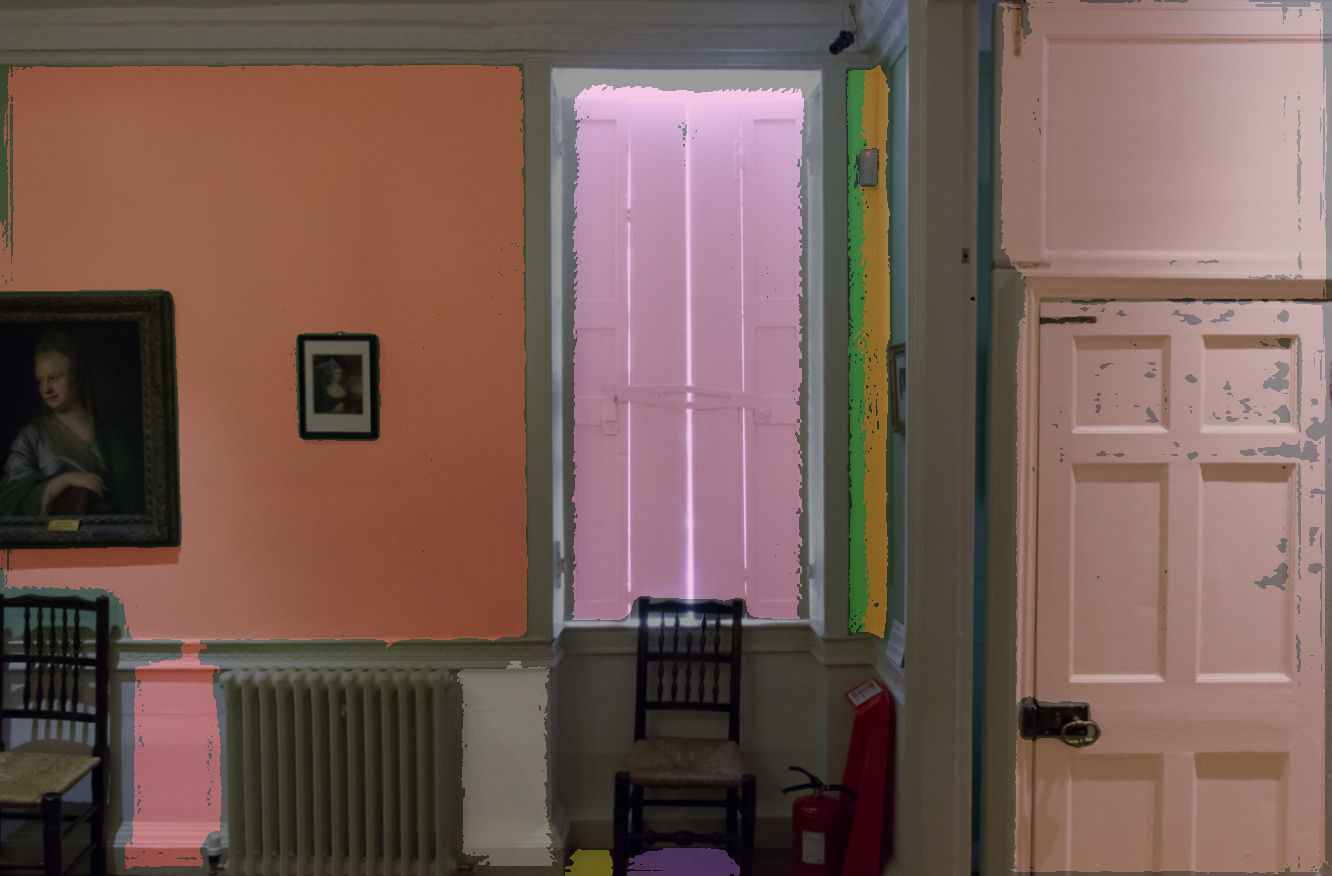
\includegraphics[width=\textwidth]{comparison_figures/planar_mask_overlay.png}
        \caption{Segmented planar regions (each colour = one plane)}
    \end{subfigure}
    \hfill
    \begin{subfigure}{0.48\textwidth}
        \centering
        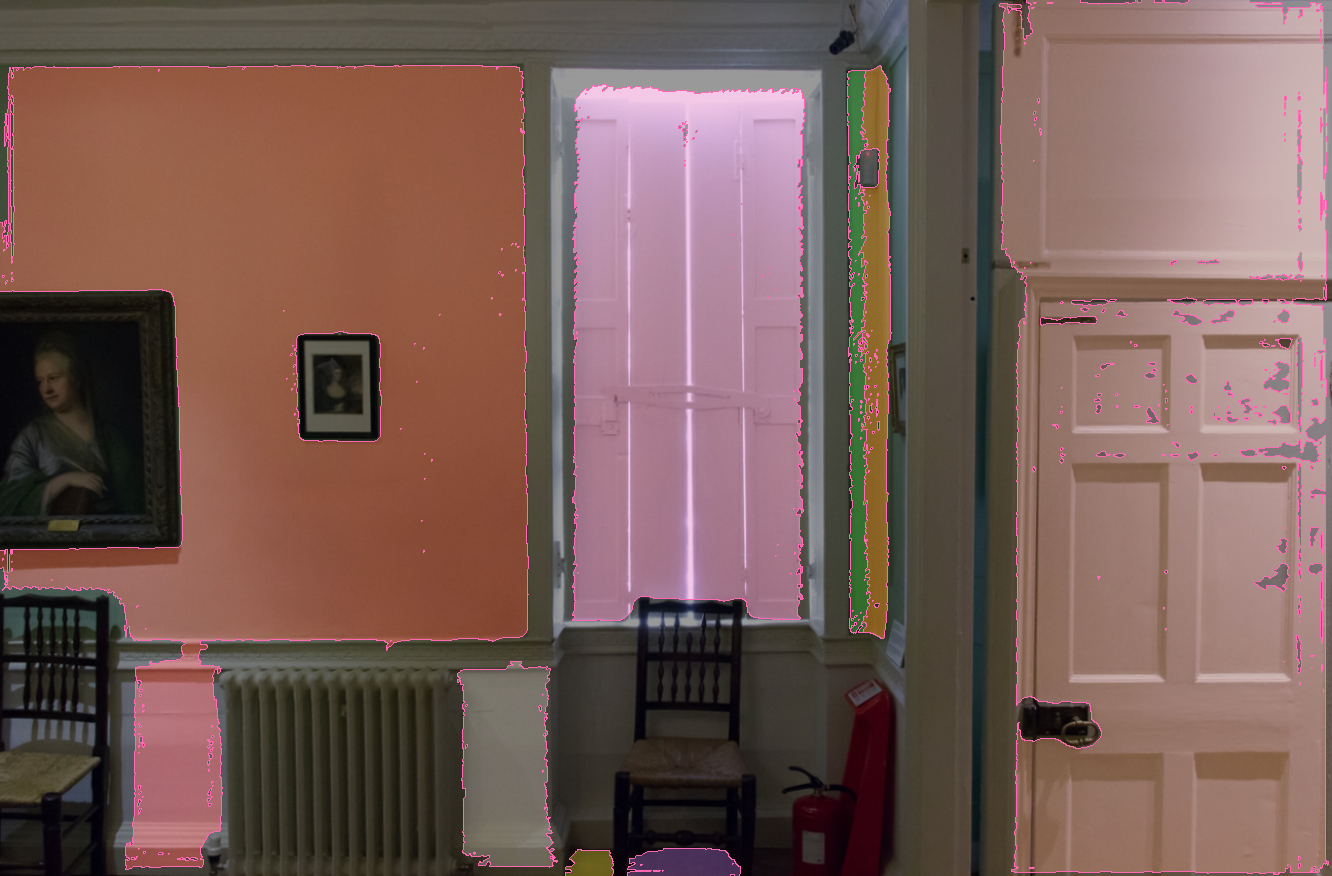
\includegraphics[width=\textwidth]{comparison_figures/plane_boundaries_pink.png}
        \caption{Plane boundaries extracted from segmentation}
    \end{subfigure}
    \caption{Planar segmentation on a DrJohnson training view.}
    \label{fig:planar_segmentation}
\end{figure}

\subsection{Edge-Aware Adaptive Representation}
\label{sec:edge_aware}

In addition to geometric priors, we introduce a spatially adaptive densification mechanism. The core intuition is straightforward: structural boundaries between planes require precise, fine-grained representation, while large homogeneous planar interiors can be covered efficiently with fewer, larger primitives.

Structural edges are identified from SAM3 planar segment boundaries, which naturally encode geometric discontinuities in the scene. Based on each Gaussian's 3D distance to these boundaries, the optimization applies two complementary rules:

\begin{itemize}
    \item \textbf{Near structural edges:} densification is boosted (split probability multiplied by $\times$2.5) and scale is capped small ($s_{\min} = 0.3$), producing many precise, localized Gaussians that capture sharp transitions faithfully.
    \item \textbf{In planar interiors:} densification is suppressed (split probability reduced by $\times$0.4) and Gaussians are free to grow large ($s_{\max} = 2.0$), covering large flat surfaces with far fewer primitives.
\end{itemize}

This allocation strategy concentrates representational capacity exactly where geometric detail is required, while preventing over-densification in uniform regions — the primary mechanism behind the model size reduction achieved by our method.

Figure~\ref{fig:edge_detection} shows the structural edge detection applied to the same DrJohnson training view. The left subfigure overlays the detected plane boundary lines on the original image; the right subfigure shows the resulting structural line segments after post-processing. Gaussians whose 3D centers project close to these lines receive boosted split probability and a tighter scale constraint, while Gaussians in the flat interiors between lines are allowed to grow large and are split less aggressively.

\begin{figure}[h]
    \centering
    \begin{subfigure}{0.48\textwidth}
        \centering
        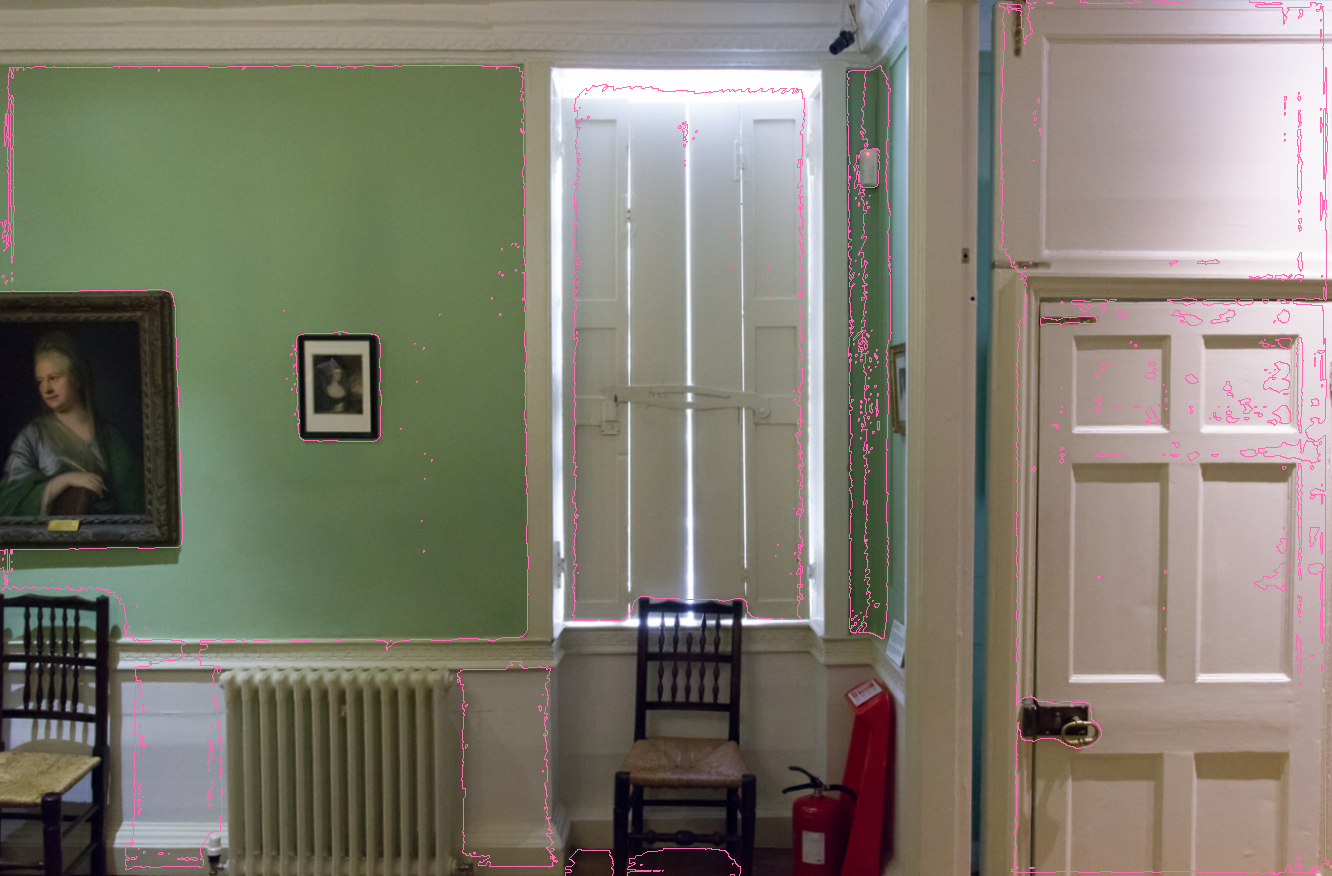
\includegraphics[width=\textwidth]{comparison_figures/edge_boundaries_on_image.png}
        \caption{Plane boundary lines overlaid on scene}
    \end{subfigure}
    \hfill
    \begin{subfigure}{0.48\textwidth}
        \centering
        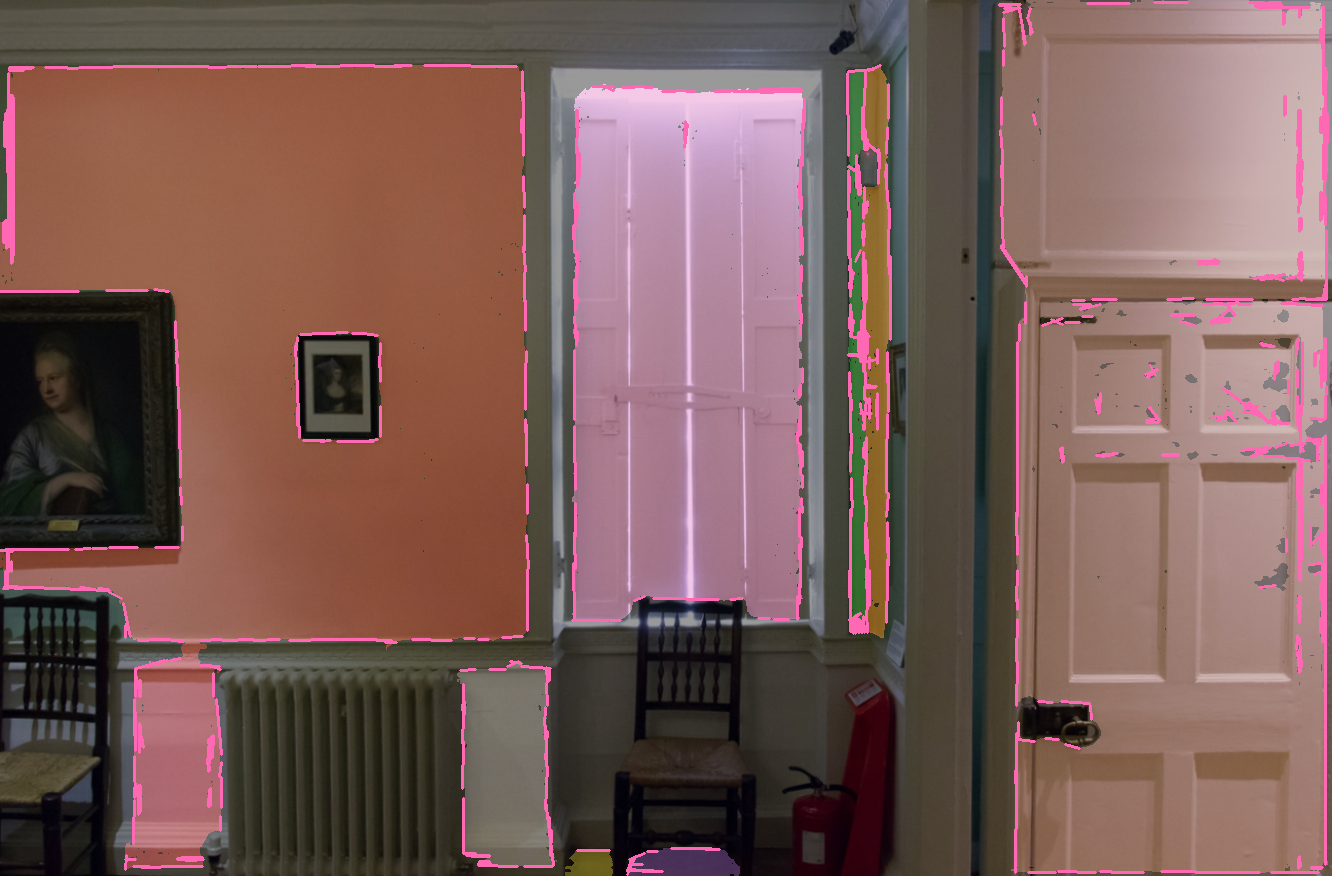
\includegraphics[width=\textwidth]{comparison_figures/edge_extracted_lines.png}
        \caption{Extracted structural line segments}
    \end{subfigure}
    \caption{Structural edge detection on a DrJohnson training view.}
    \label{fig:edge_detection}
\end{figure}

\subsubsection{Edge-Specific Normal Reinforcement}
\label{sec:edge_prior}

Optionally, an additional edge-restricted normal alignment term can be activated:

\begin{equation}
\mathcal{L}_{edge}
=
\left\|
N_r - N_{depth}
\right\|_1
+
\left(1 - N_r \cdot N_{depth} \right).
\end{equation}

This term is applied only at detected edge pixels and introduced after initial geometric stabilization to reinforce sharp transitions.

\section{Solution Summary}

The proposed framework augments standard Gaussian Splatting with:

\begin{itemize}
    \item Rendering-space geometric regularization (depth, normals, planarity),
    \item Edge-aware adaptive densification,
    \item Optional mesh-based TSDF regularization.
\end{itemize}

The design preserves the efficiency and differentiability of the original pipeline while improving geometric consistency, structural sharpness, and representation compactness.

All components are integrated into a unified training framework, enabling systematic evaluation of geometric priors and adaptive primitive allocation within a single optimization process.
